\documentclass[10pt,twocolumn]{article}

\usepackage[margin=0.72in,columnsep=0.24in]{geometry}
\usepackage{amsmath,amssymb,bm}
\usepackage{booktabs}
\usepackage{microtype}
\usepackage{xcolor}
\usepackage{hyperref}
\usepackage{enumitem}
\usepackage{graphicx}

\hypersetup{
  colorlinks=true,
  linkcolor=blue!55!black,
  citecolor=blue!55!black,
  urlcolor=blue!55!black
}
\setlist{nosep,leftmargin=*}
\newcommand{\method}{\textsc{SceneLM}}
\newcommand{\proofsys}{\textsc{SceneProof}}
\newcommand{\paperthirty}{\textsc{Paper30}}
\newcommand{\TBD}{\textcolor{red!70!black}{\textbf{TBD}}}

\newcommand{\LegacySFourSeconds}{677.77}
\newcommand{\FixSixtyOneSeconds}{192.93}
\newcommand{\FixSixtyOneSpeedup}{3.513}
\newcommand{\FixOneFourteenSeconds}{166.33}
\newcommand{\FinalSFourSeconds}{359.26}
\newcommand{\FinalSFourSpeedup}{1.887}
\newcommand{\FinalRenderWallSeconds}{415.57}

\title{From Support-Aware Recovery to Certifiable Fast Refinement:\\
\method{} and \proofsys{} for Vision-Guided 3D Scene Layouts}
\author{Anonymous Authors\\
\small Draft for internal review; author list and affiliations to be finalized}
\date{Draft: August 13, 2026}

\begin{document}
\maketitle

\begin{abstract}
Recovering an editable 3D scene from one image requires more than recognizing
objects: the result must preserve support hierarchies, image evidence, and
physical plausibility while remaining fast enough for content-production
workflows.  We build on the vision-guided Imaginarium pipeline and make two
successive contributions.  First, a support-aware recovery stage combines
visual overlap, retrieved-geometry proximity, conservative semantic routing,
and stack-aware refinement to repair unreliable support parents.  Second, we
replace 5,000-step simulated annealing with \method{}, a relation-conditioned
Levenberg--Marquardt optimizer on independent $\mathrm{SO}(3)$ tangent blocks
and support/plane translation charts.  A typed Relation Program binds every
residual to declared objects and physical witnesses; safe leaf translations
are Schur-eliminated, while \proofsys{} checks Jacobian ownership,
stationarity, contact, collision, boundary, semantic, and image-space
non-regression before component-wise commit or rollback.  On a 30-scene
benchmark evaluated on objects with at least 8,000 visible pixels, the
support-aware V3 variant obtains the highest recovery rate (91.40\%).  V5-fast
preserves the pose quality of its DeepSearch upstream source (31.34\% to
31.38\% rotation AUC and 12.19\% to 12.14\% translation AUC) while improving
the physical macro score from 54.58\% to 62.10\%.  Its final SceneLM plus
SceneProof S4 takes 359.26~s/scene, a $1.887\times$ speedup over legacy S4;
the V5-fast SceneLM/Fix61 core alone takes 192.93~s/scene.  Including measured
cold S0--S3 compute gives 829.88~s/scene for V5-fast and 996.21~s/scene for
V5-medium.  A systematic iteration-budget study yields our most instructive
negative result: raising the solver budget from two to four, eight, or sixteen
steps monotonically \emph{reduces} the equal-weight macro score, and neither
trust-region tightening nor explicit warm-start regularization recovers the
loss.  We show this is structural rather than a tuning failure---three of the
four scored families are anchored to the initialization, so the two-step
operating point acts as an implicit trust region.  We finally outline V5-best,
which selects among three cold starts using observable certificates rather
than ground truth.
\end{abstract}

\section{Introduction}

Single-image 3D scene reconstruction is attractive for games, simulation, and
digital-content creation because an image is a compact and intuitive design
interface.  The difficulty is that a visually plausible image underdetermines
the scene: object identity, canonical asset frame, depth, scale, support
parent, attachment side, and collision-free placement must all be inferred.
Errors are coupled.  A retrieved mesh with a different origin or aspect ratio
changes the pose that best explains the image; an incorrect support parent can
then make a locally plausible transform physically impossible.

Imaginarium~\cite{zhu2025imaginarium} established a strong vision-guided
foundation: it expands prompts into images, parses visual and geometric
evidence, retrieves assets, estimates poses, and refines an editable 3D
layout.  We retain this overall decomposition and focus on a narrower systems
question: \emph{how can support reasoning and final layout refinement become
faster, more auditable, and fail-closed without sacrificing the recovered
image evidence?}

Our development proceeds in two stages.  V3 introduces support analysis before
and during refinement.  It verifies declared parents with retrieved geometry,
detects plausible stacks, and conservatively reparents only candidates that
pass geometric and semantic gates.  V5 then replaces legacy simulated
annealing (SA) with \method{}, a small-iteration nonlinear least-squares solver
whose coordinates are compiled from relations.  Its companion, \proofsys{},
does not claim a formal proof of global optimality.  Instead, it emits an
executable certificate: each accepted edit is backed by declared witnesses,
checked physical and visual inequalities, and byte-safe rollback state.

The final pipeline also integrates a DeepSearch retrieval path contributed by
our advisor's team at Tencent.  DeepSearch is a production-grade asset
retriever: it indexes a library on the order of $10^5$ assets and returns the
most relevant candidates in under one second per query, which makes exhaustive
per-object retrieval affordable inside an interactive pipeline.  This
contribution is upstream of our \method{}/\proofsys{} backend and is attributed
separately throughout the paper.
Our cached results reveal an important distinction: DeepSearch preserves high
object recovery but changes retrieved asset frames and parent statistics,
which coincides with lower absolute pose AUC.  Because V4-deepsearch and
V5-fast share frozen upstream outputs and have nearly identical pose metrics,
the large V3-to-V4 pose change cannot be attributed to \method{} or
\proofsys{}.  A seed-locked S2-only ablation remains necessary for strict
causal attribution.

Code, the hosted service, and reproduction scripts are public.\footnote{Code:
\url{https://github.com/hanshengzhu0001/Lumenarium}. Project page:
\url{https://hanshengzhu0001.github.io/Lumenarium/}. Hosted system:
\url{https://embedding.lightart.qq.com/}. Asset library and derived data:
\url{https://huggingface.co/datasets/HiHiAllen/Imaginarium-Dataset} and
\url{https://huggingface.co/datasets/binicey/Imaginarium-3D-Derived-Dataset}.}

Our contributions are:
\begin{itemize}
  \item a conservative support-analysis route that combines 2D overlap, 3D
  contact proximity, semantic exclusions, and stack-aware optimization;
  \item a typed Relation Program that compiles support, plane attachment,
  containment, collision exclusion, alignment, and semantic relations into
  owned residual and certificate channels;
  \item a relation-conditioned $\mathrm{SO}(3)$ Levenberg--Marquardt solver
  with trust regions, active coordinates, and safe Schur elimination;
  \item component-wise executable certificates and scoped rollback that
  improve physical realizability while preserving the upstream pose estimate;
  and
  \item an iteration-budget analysis showing that, when most scored families
  are anchored to the initialization, a two-step budget is the empirical
  optimum and additional optimization is strictly negative-expectation---a
  measurement-design lesson that generalizes beyond this system.
\end{itemize}

\section{Method}

\subsection{Problem formulation and pipeline lineage}

For objects $i=1,\ldots,N$, the system predicts an asset $a_i$, a rigid pose
$T_i=(R_i,t_i)\in\mathrm{SE}(3)$, and a relation graph
$\mathcal{G}=(\mathcal{V},\mathcal{E})$.  Scale is fixed after retrieval in the
V5 refinement stage.  The input image supplies object masks, camera evidence,
and visual relations; retrieved meshes supply geometric witnesses.  We use the
following lineage:
\begin{enumerate}
  \item \textbf{V1:} the original recovery and legacy SA refinement;
  \item \textbf{V3:} V1 plus support verification and stack-aware S3/S4;
  \item \textbf{V4-deepsearch:} V3 with the Tencent DeepSearch S2 retriever;
  \item \textbf{V5-fast:} frozen V4 S0--S3 followed by SceneLM/Fix61;
  \item \textbf{V5-medium:} V5-fast plus Fix114 true-mesh support/visibility
  repair; and
  \item \textbf{V5-best (planned):} three V5 cold starts followed by a
  certificate-only selector, with no access to evaluation ground truth.
\end{enumerate}

\subsection{Support-aware recovery (V1 $\rightarrow$ V3)}

Let $u$ be a proposed upper object and $\ell$ a lower support.  A broad stack
detector first evaluates image-space horizontal overlap
\begin{equation}
  o_x(u,\ell)=
  \frac{|I_x(u)\cap I_x(\ell)|}
       {\min(|I_x(u)|,|I_x(\ell)|)}
\end{equation}
and retrieved-geometry vertical contact
\begin{equation}
  \delta_y(u,\ell)=y_{\mathrm{bottom}}(u)-y_{\mathrm{top}}(\ell).
\end{equation}
A candidate must satisfy an overlap threshold, a depth-interval tolerance, the
ordering $y_{\mathrm{center}}(u)<y_{\mathrm{center}}(\ell)$ in the pipeline's
camera convention, and asymmetric penetration/gap bounds on $\delta_y$.  Among
valid supports, the detector chooses the smallest $|\delta_y|$.

Detection is deliberately broader than mutation.  A conservative gate rejects
anonymous objects, wall/ceiling attachments, non-floor parents that disagree
with the proposal, implausible semantic roles, and oversized upper objects.
Only small cargo-like uppers on support-like lowers are reparented by the strong
stack route; ordinary tabletop relations retain their existing parent.  S4
then optimizes with the accepted stack edge active.  This separation between
\emph{candidate discovery} and \emph{mutation authority} prevents a noisy 2D
coincidence from rewriting the support tree.

\subsection{Typed Relation Programs}

V5 compiles each scene into a deterministic Relation Program bundle.  A
program $p$ declares: (i) participating object/part witnesses, (ii) owned
variable blocks, (iii) a robust residual channel for the solver, and (iv) an
independent measurement and threshold for certification.  Supported program
kinds include
\begin{equation}
\begin{aligned}
\{&\textsc{Support},\textsc{Stack},\textsc{PlaneAttach},
\textsc{CeilingAttach},\\
&\textsc{Hang},\textsc{Inside},\textsc{CollisionExclusion},\\
&\textsc{PointTowards},\textsc{Align},\textsc{Distance}\}.
\end{aligned}
\end{equation}
Every solver variable owner must be one of the factor's participants.  This
simple typing rule enables a numerical ownership audit: undeclared Jacobian
blocks must be zero up to tolerance.  Solver residuals and certificate
measurements are kept distinct so that a low optimization loss cannot silently
stand in for a physical witness.

Given robust kernels $\rho_p$, weights $W_p$, and residuals $r_p$, the compiled
objective is
\begin{equation}
  E(x)=\frac{1}{2}\sum_{p\in\mathcal{P}_{\mathrm{solver}}}
  \rho_p\!\left(\|W_p^{1/2}r_p(x)\|_2^2\right).
  \label{eq:objective}
\end{equation}
Hard relations additionally create proof obligations even when they are not
used as smooth solver factors.

\subsection{Relation-conditioned pose coordinates}

Each non-rigid object owns an independent world-frame rotation tangent
$\omega_i\in\mathbb{R}^3$:
\begin{equation}
  R_i(\omega_i)=\exp([\omega_i]_{\times})\bar R_i,
  \label{eq:so3}
\end{equation}
where $\bar R_i$ is the frozen warm start.  The exponential uses Rodrigues'
formula with a small-angle series.  Translation is expressed in a chart chosen
by the relation: world $xyz$, support $uvh$, or plane $uvn$.  If $\pi(i)$ is a
support parent, the decoded center is
\begin{equation}
  t_i=t_{\pi(i)}+\Delta R_{\pi(i)}
  (\bar t_i-\bar t_{\pi(i)})+
  \Delta R_{\pi(i)}B_iq_i,
  \label{eq:decode}
\end{equation}
where $B_i$ is the chart basis and $q_i$ its local coordinates.  Parent motion
therefore transports a child's center, while the child's orientation remains
an independent $\mathrm{SO}(3)$ block.  This avoids incorrectly inheriting a
parent's rotation.

\subsection{SceneLM: guarded Levenberg--Marquardt}

At iterate $x_k$, automatic differentiation forms $r_k$ and the block
Jacobian $J_k$.  \method{} solves
\begin{equation}
\begin{aligned}
 (J_k^\top J_k+\lambda_k D_k)\Delta x_k&=-J_k^\top r_k,\\
 D_k&=\mathrm{diag}\!\left(\max(|\mathrm{diag}(J_k^\top J_k)|,1)\right).
\end{aligned}
 \label{eq:lm}
\end{equation}
The implementation supports matrix-free $Jv/J^\top v$ products with
preconditioned conjugate gradients and an independently assembled block normal
system used for parity checks and guarded solves.  Frozen objects are masked
out of both differentiation and updates.  A global trust scale caps maximum
translation and rotation without changing the step direction.

For predicted reduction $\widehat{\Delta E}$ and actual reduction $\Delta E$,
the gain ratio is
\begin{equation}
  \gamma_k=\frac{E(x_k)-E(x_k+\Delta x_k)}
  {-[g_k^\top\Delta x_k+\tfrac12\Delta x_k^\top H_k\Delta x_k]}.
\end{equation}
The step is accepted only if it is finite, decreases the nonlinear objective,
and $\gamma_k$ exceeds a threshold.  High-ratio steps halve damping; weak
accepted steps increase it; rejected steps multiply damping by four.  This
replaces thousands of stochastic proposals with a few evidence-conditioned
iterations.

For stable leaf support blocks, only translation coordinates may be
eliminated.  Partitioning the damped normal system into retained $r$ and
eliminated $e$ variables yields
\begin{equation}
  S=H_{rr}-H_{re}H_{ee}^{-1}H_{er},\quad
  \tilde b_r=b_r-H_{re}H_{ee}^{-1}b_e.
  \label{eq:schur}
\end{equation}
Rotations are never Schur-eliminated.  A leaf is eligible only when its stable
incident factors involve the child and its declared parent; otherwise the
system keeps the full block.

\subsection{SceneProof certificates and scoped rollback}

Optimization proposes a candidate; certification decides whether it may
replace the incumbent.  The certificate records:
\begin{itemize}
  \item Jacobian ownership and block/dense normal-system parity;
  \item projected stationarity, primal residual maxima, and trust-region use;
  \item exact- or true-mesh support/contact and attachment witnesses;
  \item collision non-worsening, boundary containment, plane attachment, and
  semantic non-inferiority;
  \item image-space mask/visibility non-regression for visual repair; and
  \item pose-serialization and incumbent-restoration parity.
\end{itemize}

Let $m_c(x)$ be a higher-is-better score for component
$c\in\{\mathrm{collision},\mathrm{support},\mathrm{plane},
\mathrm{semantic},\mathrm{rotation},\mathrm{translation}\}$.  A component
passes when
\begin{equation}
  m_c(x')-m_c(x)\ge -\epsilon_c.
  \label{eq:noninferior}
\end{equation}
In addition, an incumbent hard program that passes may not become non-passing,
and a new hard failure is forbidden.  Failed program witnesses identify only
their variable owners and declared separators.  Those objects are rolled back
rather than discarding unrelated accepted components.  Missing evidence yields
\textsc{Abstain}; unresolved visible support/attachment failures are surfaced
instead of being silently labeled successful.

\subsection{Fast, medium, and best operating points}

\textbf{V5-fast} executes one cold start and \method{}/Fix61. It is the
quantitative paper default: two LM iterations, semantic weight $0.5$, and
warm-start weight $0.01$. \textbf{V5-medium} additionally executes the
conservative Fix114 true-mesh support/visibility repair layer; it is a
presentation profile and its quality row is never merged into the headline
table. \textbf{V5-best} runs three independent cold starts followed by a
selector over observable evidence: certificate coverage, hard-program status,
physical component scores, image agreement, and runtime.  Ground truth is
never a selector feature, so the profile remains a legitimate test-time
procedure rather than an oracle.  Flux fine-tuning is a separate future
upstream ablation and is not part of the reported V5-fast results.

\subsection{Early stopping as an implicit trust region}
\label{sec:earlystop}

The two-iteration budget of Fix61 deserves an explicit account, because it
looks like premature termination.  Solver diagnostics confirm it is not a
convergence event: the persisted certificate reports
\texttt{executed\_iterations}~$=2$ with \texttt{converged}~$=$~\textsc{false},
and one of the two steps is already rejected by the gain-ratio test.  The
budget is an imposed constraint, and we argue it is the correct one.

Let $\mathcal{F}=\{\mathrm{coll},\mathrm{supp},\mathrm{plane},\mathrm{sem}\}$
be the scored families and $\bar T$ the frozen warm start produced by S0--S3.
Two properties of the evaluation are decisive.  First, the semantic family is
gated on warm-start self-consistency: a declared relation enters the scored set
only if $\bar T$ already satisfies it within tolerance, so relations the
initialization violates are abstained rather than scored.  Second, the support
family is defined relative to the S3 support tree, and the plane family is
invariant to the in-plane motions the solver can express.  Writing
$m_c(\cdot)$ for the family scores, this means
\begin{equation}
  \arg\max_{T} m_c(T)\;\approx\;\bar T
  \quad\text{for } c\in\{\mathrm{supp},\mathrm{plane},\mathrm{sem}\},
  \label{eq:anchored}
\end{equation}
whereas only $m_{\mathrm{coll}}$ has its maximizer strictly away from $\bar T$
whenever the initialization contains interpenetration.  The equal-weight macro
\begin{equation}
  M(T)=\tfrac14\!\!\sum_{c\in\mathcal{F}}\!\! m_c(T)
\end{equation}
therefore decomposes into three \emph{fidelity} terms that any displacement can
only decrease and one \emph{improvement} term that displacement can increase.
Because the solver descends $E$ in \eqref{eq:objective} rather than ascending
$M$, and $E$ weights collision and contact above semantic, each additional
accepted step trades fidelity for improvement at a ratio that is unfavourable
under equal family weights.  Truncating the trajectory after two steps bounds
the achievable displacement $\|T-\bar T\|$ and thus bounds the fidelity loss:
early stopping is a trust region on the initialization, expressed in iteration
count instead of in the objective.

This account is falsifiable, and we test it three ways in
Section~\ref{sec:budget}.  If the mechanism were merely excessive per-step
rotation, capping the yaw step while keeping the total angular budget fixed
would restore the score; if it were an implicit-versus-explicit mismatch,
raising the warm-start weight $w_{\mathrm{ws}}$ in $E$ would let a larger
budget succeed.  Neither holds, which is what promotes
\eqref{eq:anchored} from a convenient story to the operative explanation.

\section{Experimental Setup}

\paragraph{Benchmark.}
We evaluate on \paperthirty{}, a fixed 30-scene set.  The headline pose
protocol includes only recovered objects whose visible S1 mask area is at
least 8,000 pixels.  We report Primary recovery, Primary support-parent
accuracy, aligned rotation AUC up to $60^\circ$, and aligned translation AUC
up to $0.5$~m.  Ground truth is used only for evaluation.

\paragraph{Physical metrics.}
The physical macro averages the applicable collision, support, plane, and
semantic families under the frozen native geometry for each version.  Boundary
is diagnostic when scene coverage is non-degenerate.  Unless explicitly
labeled relation-conditioned, the comparison uses the common legacy collision
policy.  V3's physical macro is omitted because a fresh evaluator and an older
dashboard disagree (41.20\% versus 52.14\%); publishing either before
provenance reconciliation would be misleading.

\paragraph{Runtime.}
V1 and V3 share the same legacy SA5000 runtime profile.  Twenty-seven
successful V3 per-scene records total 38,498.6~s; mean-imputing three missing
successful records gives approximately 1,425.9~s per scene, 11.9 useful
GPU-hours for \paperthirty{}, or 5.9~h ideal balanced wall time on two NVIDIA
A10 GPUs.  An additional 2.17 GPU-hours came from recorded failed retries and
is reported separately.  DeepSearch shortens S2 by roughly 80~s per scene, so
we report V4-deepsearch as approximately 1,345.9~s per scene (11.2 GPU-hours,
or 5.6 ideal two-A10 hours), rather than as a precision timing claim.
For S4 alone, the latest same-input Paper30 record is 677.77~s/scene for
legacy SA5000 and approximately 192.93~s/scene for Fix61, a $3.513\times$
speedup.  The conservative Fix114 support/visibility layer adds 166.33~s per
scene, giving 359.26~s/scene and a $1.887\times$ final S4 speedup.  A final
30-scene, 256-sample rendering pass takes 415.57~s wall time on two A10s and is
reported separately from S4.  The Fix61 result supersedes an earlier
intermediate measurement of 218.80~s/scene ($3.10\times$).  Cold S0--S3 uses
636.95~s/scene (5.308 GPU-hours), with 2.680~h measured wall time on two A10s.
Its measured per-scene decomposition is S0 9.69~s, S1 443.04~s, S2 137.45~s,
S3 44.79~s, and orchestration overhead 1.99~s. These terms close exactly to
636.95~s; S1 accounts for 69.6\% of S0--S3 compute and is the dominant
full-chain bottleneck.
Thus V5-fast S0--S4 uses 829.88~s/scene (6.916 GPU-hours; 3.458 ideal balanced
two-A10 hours), while V5-medium uses 996.21~s/scene (8.302 GPU-hours; 4.151
ideal balanced two-A10 hours). Ideal-balanced values are compute
normalizations, not observed full-chain wall times.

\section{Results}

\begin{table*}[t]
\centering
\caption{Primary 8,000-pixel pose results and frozen physical scores on
\paperthirty{}.  The V3 physical value is withheld pending provenance
reconciliation.  Best values are bold.}
\label{tab:quality}
\small
\begin{tabular}{lccccc}
\toprule
Version & Recovery $\uparrow$ & Parent $\uparrow$ & Rot. AUC@60 $\uparrow$ &
Trans. AUC@0.5 $\uparrow$ & Physical macro $\uparrow$ \\
\midrule
V1 & 89.49 & \textbf{89.32} & \textbf{48.13} & \textbf{23.73} & 52.98 \\
V3 support-aware & \textbf{91.40} & 87.80 & 48.11 & 20.36 & under audit \\
V4-deepsearch & 88.22 & 80.14 & 31.34 & 12.19 & 54.58 \\
V5-fast & 88.22 & 80.14 & 31.38 & 12.14 & \textbf{62.10} \\
\bottomrule
\end{tabular}
\end{table*}

\subsection{Support analysis improves recovery}

V3 reaches the highest Primary recovery, 91.40\%, an absolute gain of
1.91 points over V1.  The result does not dominate every pose metric: parent
accuracy decreases by 1.52 points and translation AUC by 3.37 points, while
rotation is essentially unchanged.  The correct conclusion is therefore that
support-aware routing recovers more visible instances and supplies useful
stack structure, not that it universally solves pose estimation.  The
conservative mutation gate is important: the geometric detector is noisy, and
unrestricted reparenting would trade recovery for incorrect support edges.

\subsection{SceneLM/SceneProof improves physics without causing the pose drop}

V5-fast improves the physical macro from 54.58\% to 62.10\% relative to its
actual upstream source, V4-deepsearch, a gain of 7.52 points.  At the same time,
rotation changes by only $+0.04$ points and translation by $-0.05$ points.
Thus the backend's physical gain is not obtained by a substantial change in
headline pose quality.

The much larger V3-to-V4 changes occur before \method{}: rotation falls by
16.77 points, translation by 8.17 points, and parent accuracy by 7.66 points.
The defining lineage change is the S2 retriever.  DeepSearch can select assets
with different canonical axes, origins, scales, aspect ratios, and footprints;
these alter both pose evaluation and downstream parent geometry.  This is
strong attribution evidence but not a strict causal proof, because the cached
V3 and V4 runs were not generated with an identical S1 state and seed while
toggling only S2.

\begin{table}[t]
\centering
\caption{Runtime accounting with distinct scopes.  End-to-end V1/V3 is
reconstructed from 27/30 successful timing rows; V4 subtracts the observed
${\sim}80$~s/scene S2 saving.  V5-fast reports the measured final S4 and its
components.  The interrupted Fix124 coordinator completed S0--S3 for 30/30
scenes but did not emit a trustworthy combined cold-start wall-time summary.}
\label{tab:runtime}
\small
\begin{tabular}{lccc}
\toprule
Scope & Mean/scene & Paper30 GPU-hours & Speedup \\
\midrule
V1/V3 full chain (reconstructed) & ${\sim}1{,}425.9$ s & ${\sim}11.9$ h & reference \\
V4-deepsearch full chain (approx.) & ${\sim}1{,}345.9$ s & ${\sim}11.2$ h & ${\sim}1.06\times$ \\
Legacy S4 / SA5000 & 677.77 s & 5.65 h & reference \\
SceneLM / Fix61 core & 192.93 s & 1.61 h & $3.513\times$ \\
SceneProof / Fix114 add-on & 166.33 s & 1.39 h & additive \\
V5-medium final S4 & \textbf{359.26 s} & \textbf{2.99 h} & \textbf{$1.887\times$} \\
V5-fast S0--S4 compute & 829.88 s & 6.92 h & --- \\
V5-medium S0--S4 compute & 996.21 s & 8.30 h & --- \\
\bottomrule
\end{tabular}
\end{table}

\subsection{The iteration budget is already optimal at two steps}
\label{sec:budget}

Section~\ref{sec:earlystop} predicts that additional solver budget is
negative-expectation under an equal-weight macro whose majority of families is
anchored to the warm start.  Table~\ref{tab:budget} reports the test on a
five-scene subset (\textsc{bedroom\_01}, \textsc{livingroom\_10},
\textsc{casino\_01}, \textsc{official\_01}, \textsc{streetlitter\_01}) with the
S3 source, geometry, and evaluator frozen; only the S4 configuration varies.

Three findings follow.  First, budget alone is harmful and the damage is
front-loaded: the semantic family falls from 0.7634 at two steps to 0.5209 at
four and then saturates at 0.5210 by eight, so the optimum at two steps is a
cliff edge rather than the peak of a smooth curve.  Second, the collision
family---the only one whose maximizer lies away from $\bar T$---does improve
with budget (0.4301 to 0.4436), exactly as \eqref{eq:anchored} predicts, but
its $\tfrac14$ weight cannot pay for the fidelity loss.  Third, both proposed
rescues fail.  Reducing the per-step yaw cap from $15^\circ$ to $3.75^\circ$
while raising the step count from two to eight holds the total angular budget
fixed at $30^\circ$ and recovers only $63\%$ of the semantic deficit, while
support degrades further because the trust region reallocates the step into
translation; additionally tightening the translation cap to $0.05$~m loses the
recovered semantic again.  Raising $w_{\mathrm{ws}}$ from $0.01$ to $0.3$ is
worse than doing nothing.  We also verified that the horizontal
footprint-containment residual is \emph{already} present in $E$ with unit
weight, so the support degradation is not an omitted-term artifact.

Two caveats bound this claim.  The comparison is over a step-count, step-cap,
and weight grid, not over all conceivable regularizers; and the conclusion is
stated with respect to \emph{this} equal-weight macro, which by construction
rewards agreement with the initialization on three of four families.  A
metric that weighted collision more heavily, or that scored semantic relations
the initialization violates, would move the optimum.

\begin{table}[t]
\centering
\caption{Iteration-budget frontier on the five-scene subset with frozen S3
geometry and evaluator.  All arms use the second-order \method{} solver; only
the S4 configuration varies.  The two-step Fix61 operating point is optimal in
macro, and every attempt to spend more budget profitably fails.}
\label{tab:budget}
\small
\begin{tabular}{lcccc}
\toprule
S4 configuration & macro $\uparrow$ & coll. & supp. & sem. \\
\midrule
Fix61: 2 steps (default) & \textbf{0.6183} & 0.4301 & \textbf{0.5684} & \textbf{0.7634} \\
4 steps & 0.5782 & 0.4394 & 0.5459 & 0.5209 \\
8 steps & 0.5828 & \textbf{0.4436} & 0.5480 & 0.5210 \\
8 steps, yaw cap $3.75^\circ$ & 0.6004 & 0.4380 & 0.5391 & 0.6741 \\
8 steps, yaw $3.75^\circ$ + trans. $0.05$ m & 0.5799 & 0.4304 & 0.5495 & 0.5943 \\
8 steps, $w_{\mathrm{ws}}=0.3$ & 0.5672 & 0.4130 & 0.5510 & 0.4563 \\
\bottomrule
\end{tabular}
\end{table}

\subsection{Second-order robustness}

A first-order Adam variant with hard projection reaches a higher single-scene
macro than \method{} (0.6822 versus 0.6338 at its own best budget), but it does
not complete the five-scene subset: on \textsc{official\_01}, a 112-object
scene with fourteen support footprints whose initial error exceeds $0.5$~m, the
half-space projection has no feasible point and the stage aborts.  \method{}
completes all five scenes because infeasible relations enter as weighted
residuals and, when necessary, are released by the bounded relation-release
mechanism rather than raising.  Relative to legacy SA5000, the second-order
solver improves the collision family from 0.3719 to 0.4301 ($+15.6\%$
relative).  We therefore treat robustness, not single-scene optimality, as the
operative argument for the second-order path.

\begin{figure*}[t]
\centering
\begin{tabular}{cccc}
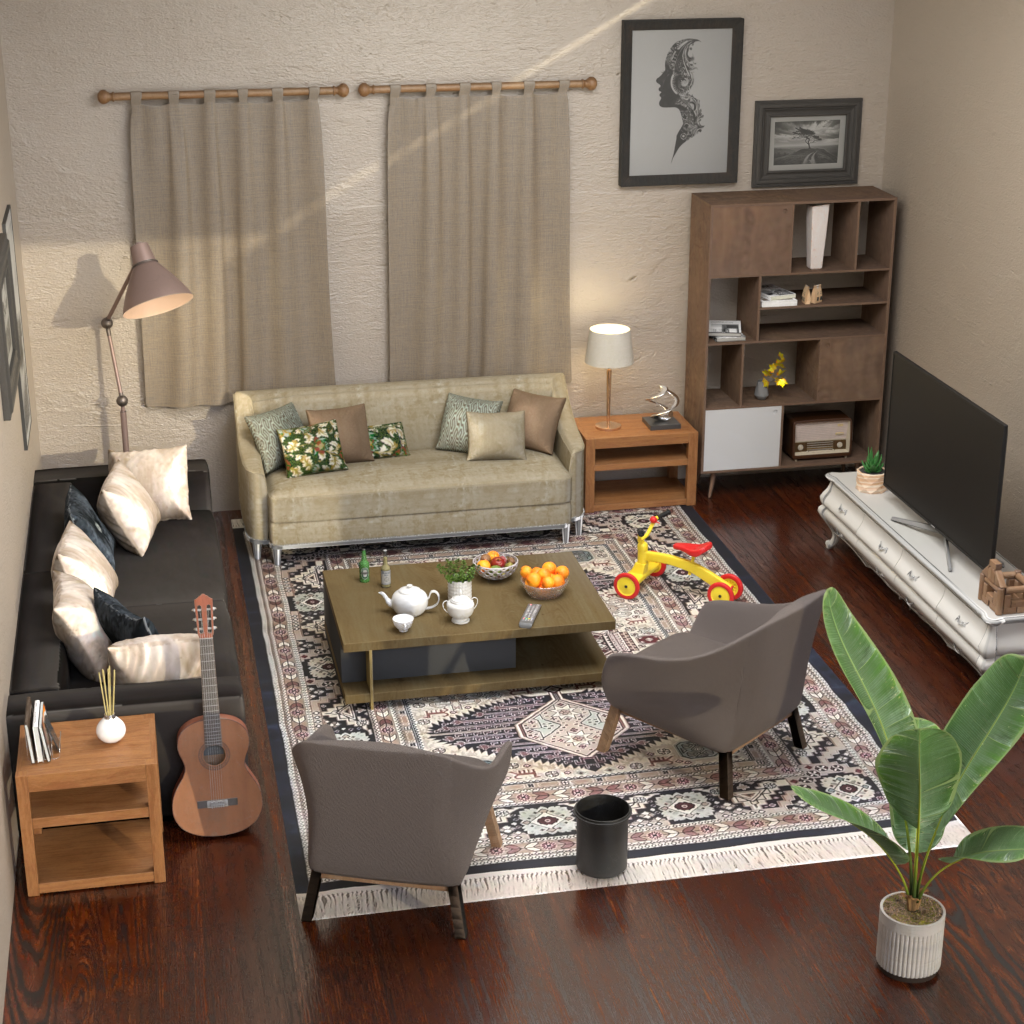
\includegraphics[width=0.235\textwidth]{../visual_results/livingroom_10_worst_input.png} &
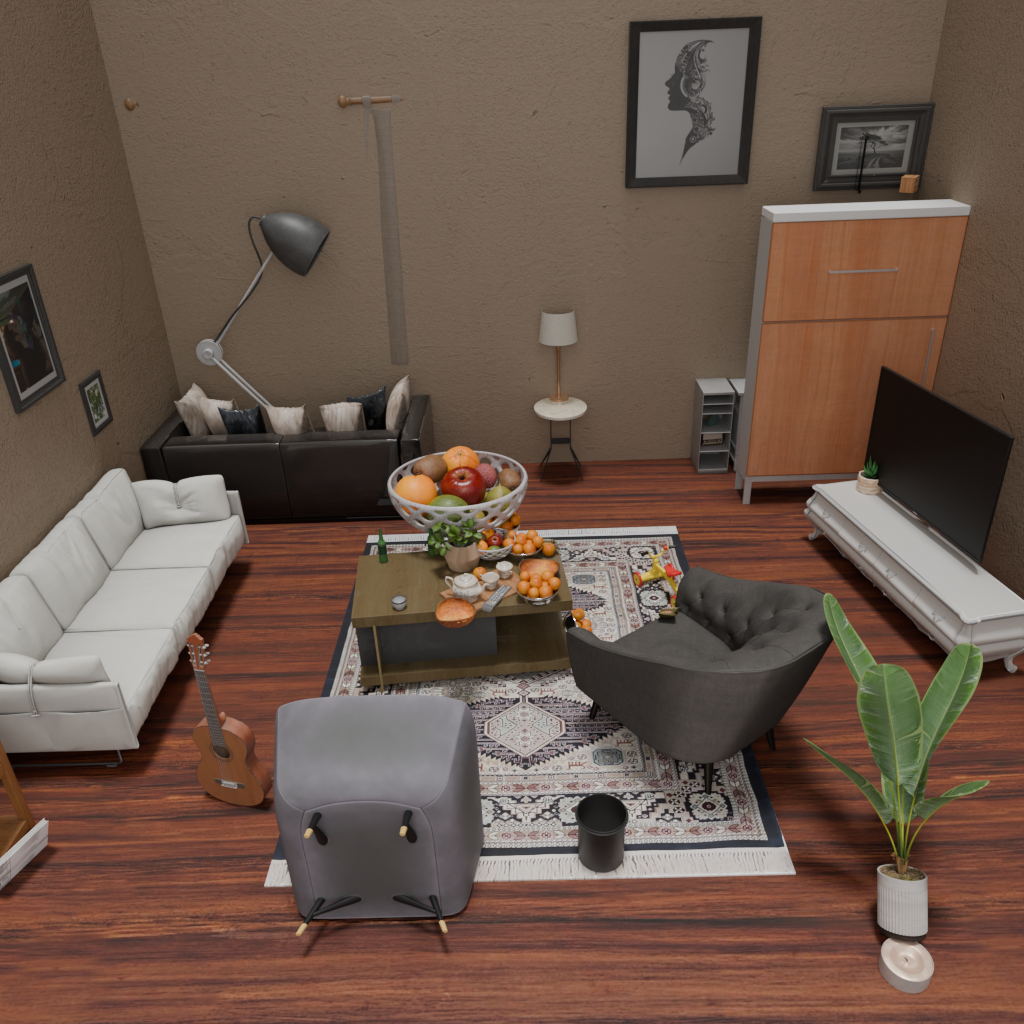
\includegraphics[width=0.235\textwidth]{../visual_results/livingroom_10_worst_v1_final.png} &
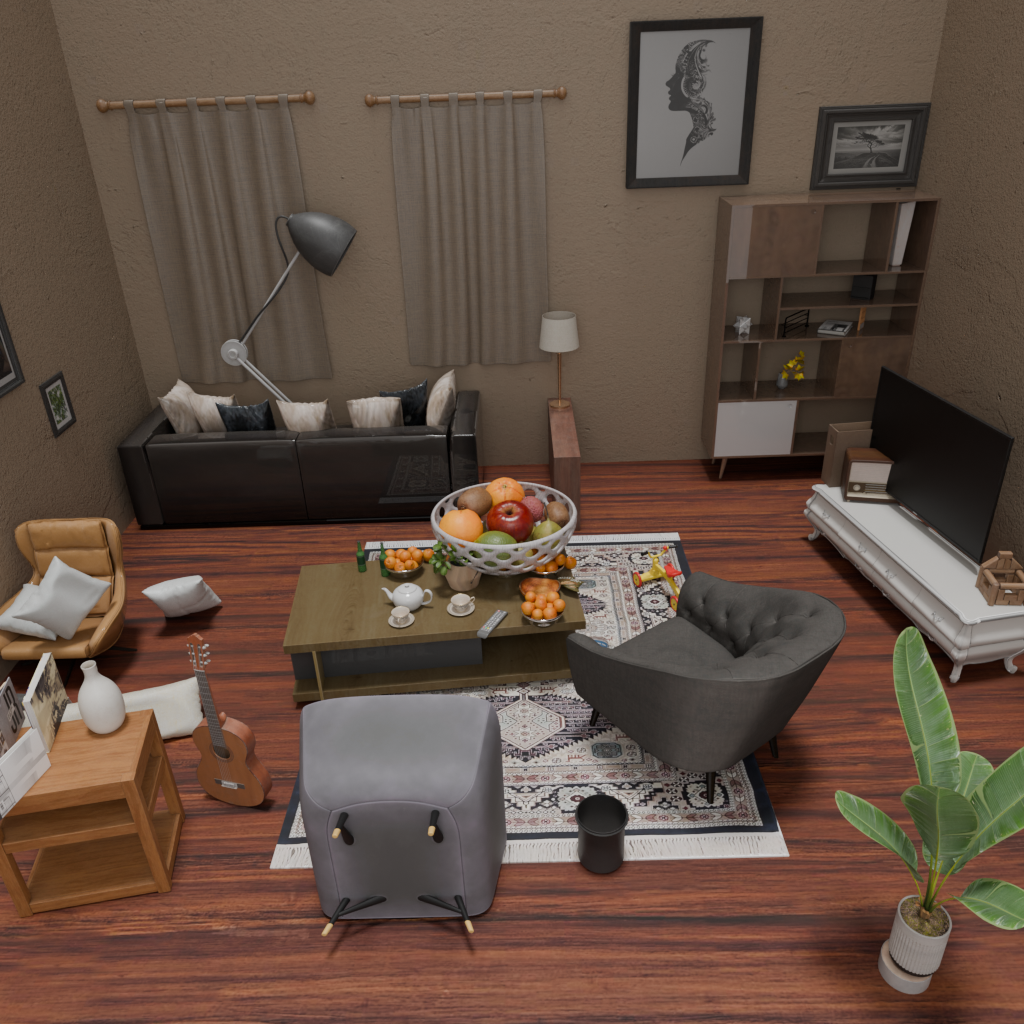
\includegraphics[width=0.235\textwidth]{../visual_results/livingroom_10_worst_v3_final.png} &
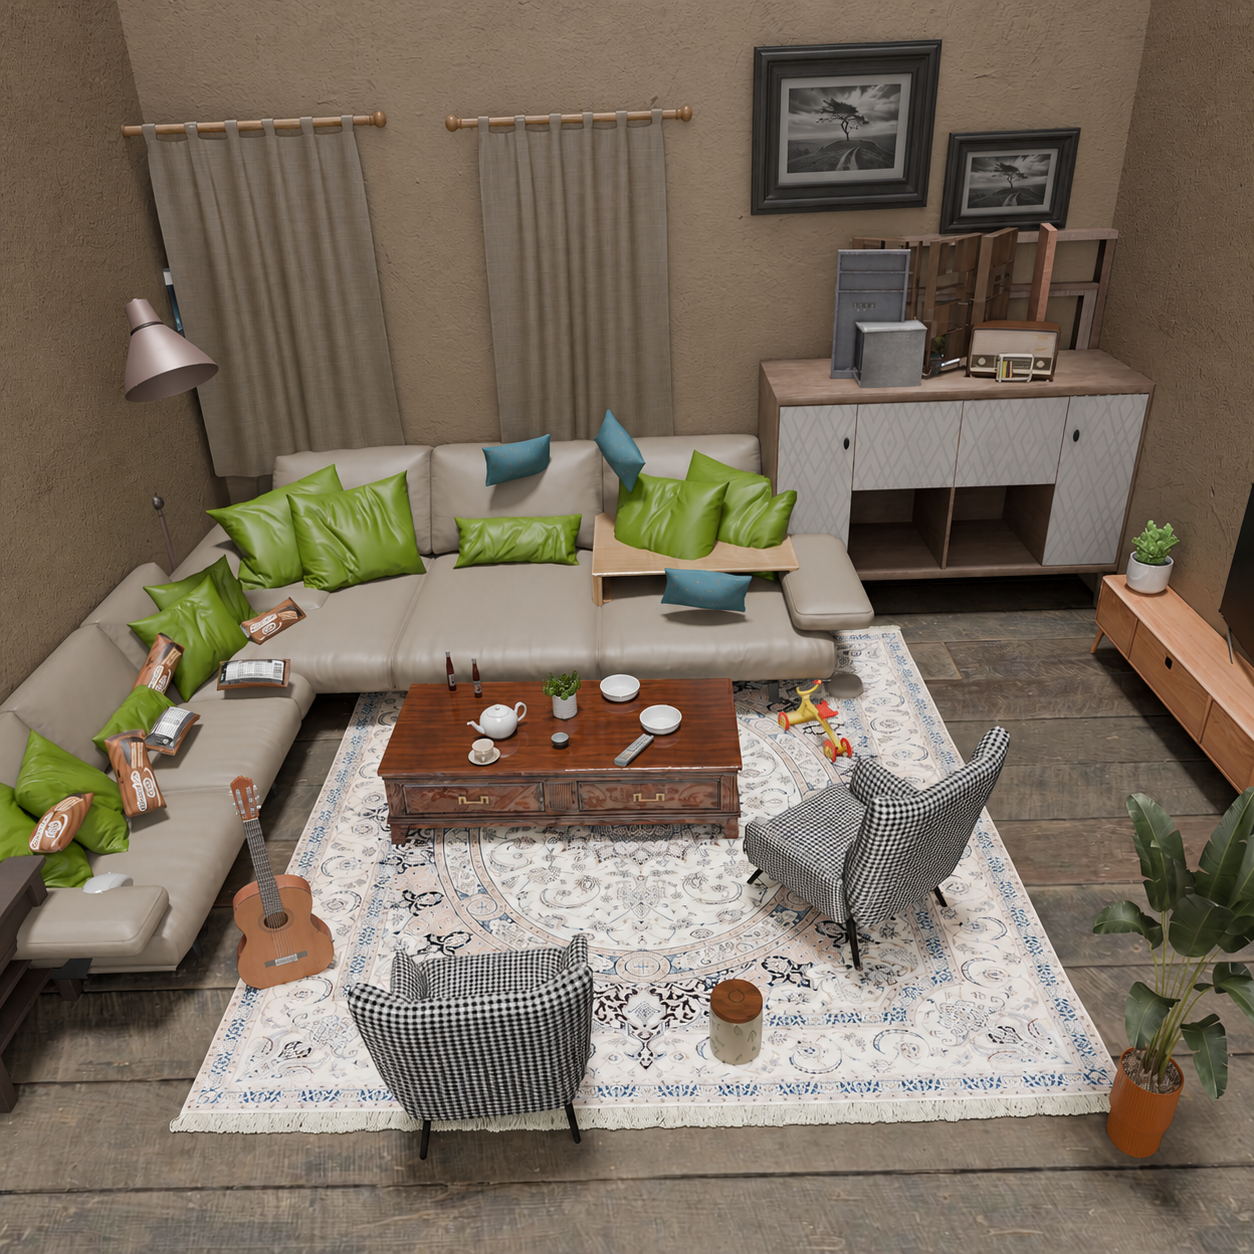
\includegraphics[width=0.235\textwidth]{../visual_results/livingroom_v5_final.png} \\
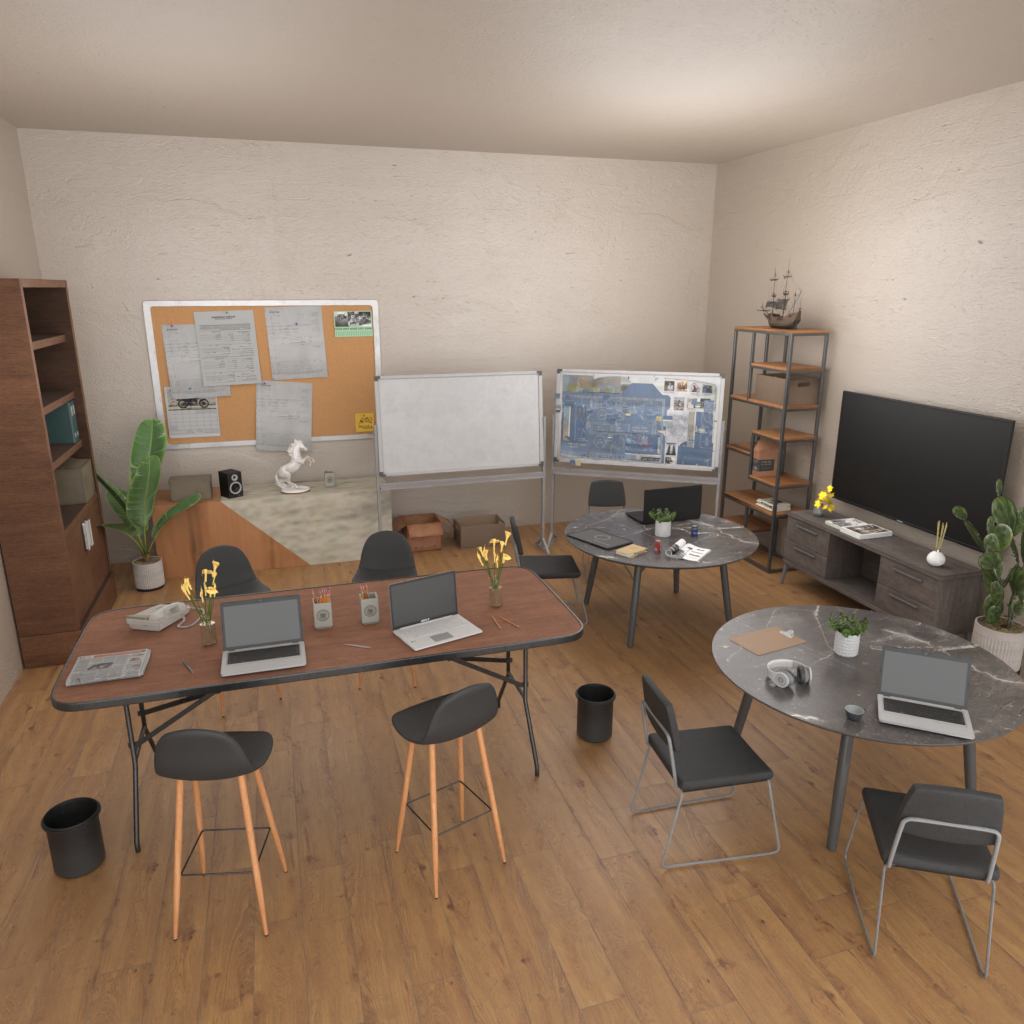
\includegraphics[width=0.235\textwidth]{../visual_results/official_02_worst_input.png} &
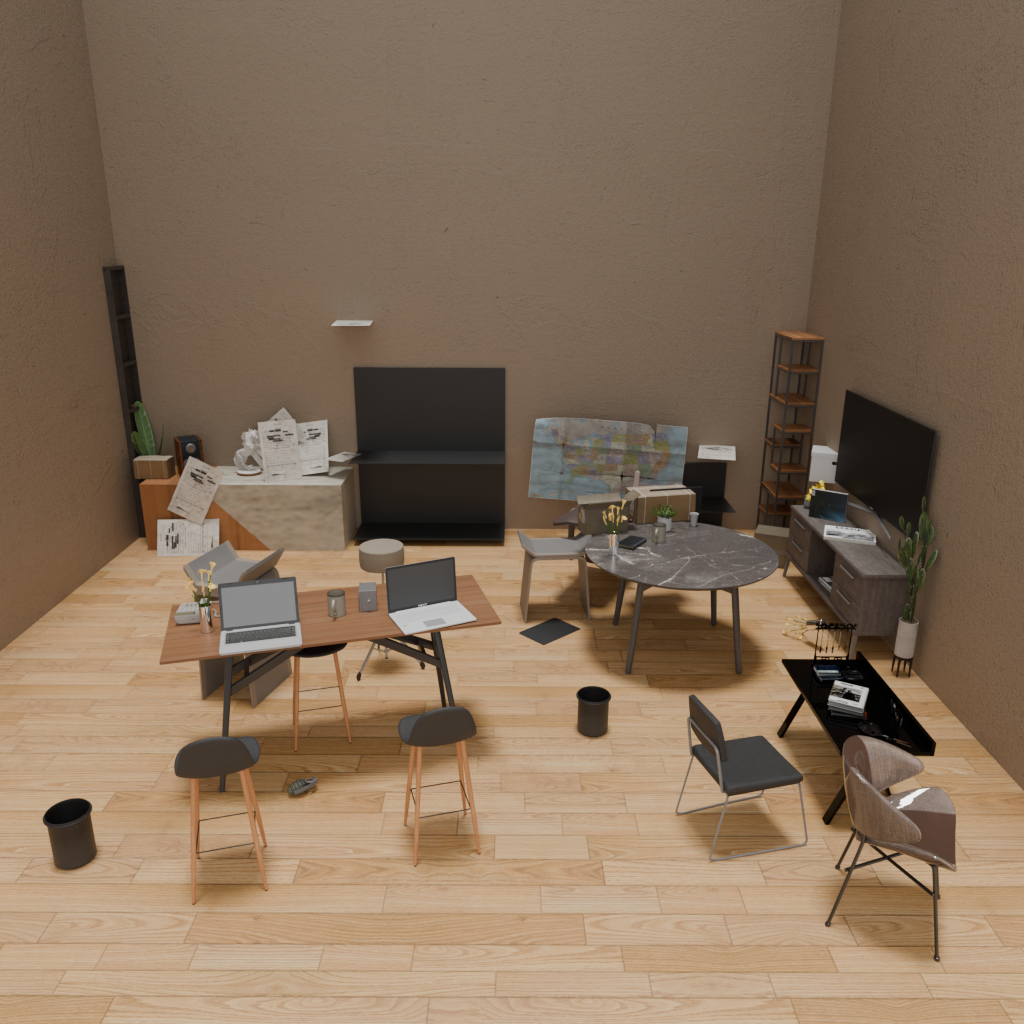
\includegraphics[width=0.235\textwidth]{../visual_results/official_02_worst_v1_final.png} &
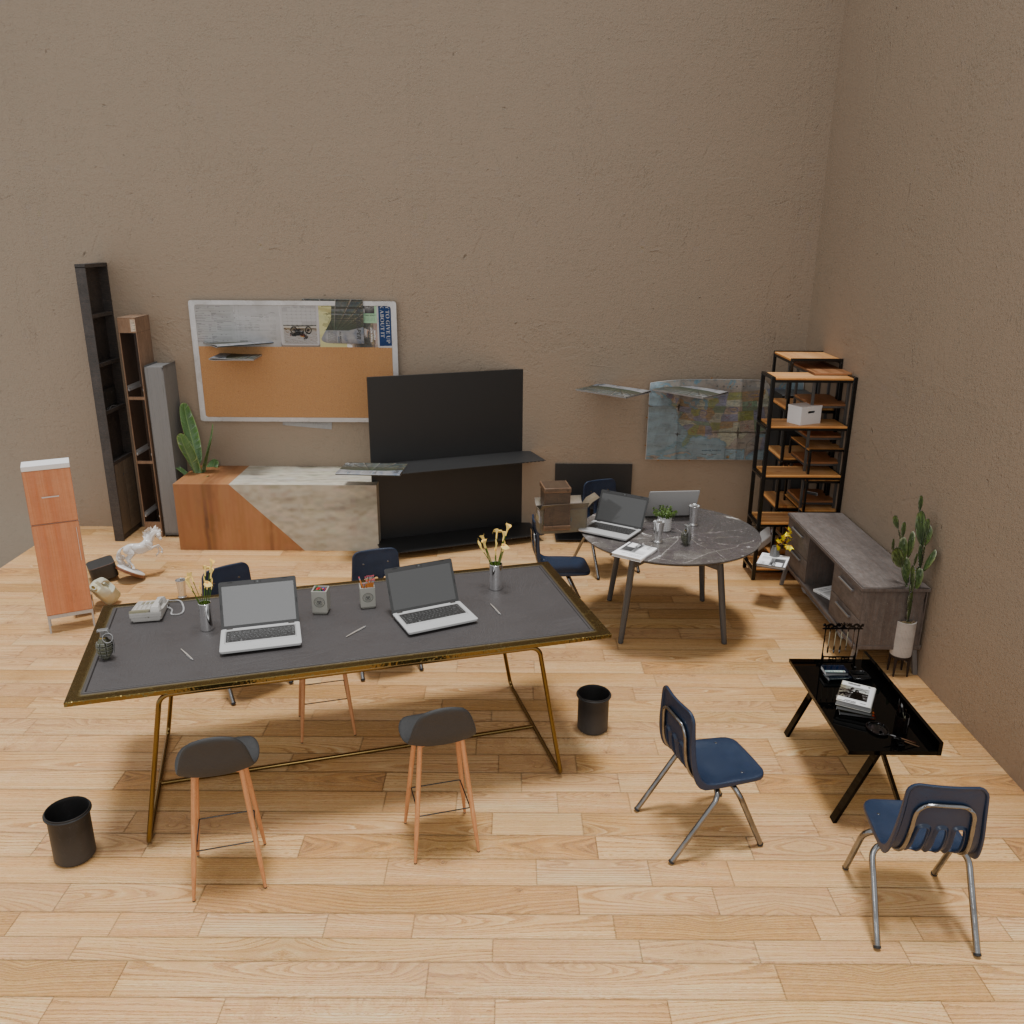
\includegraphics[width=0.235\textwidth]{../visual_results/official_02_worst_v3_final.png} &
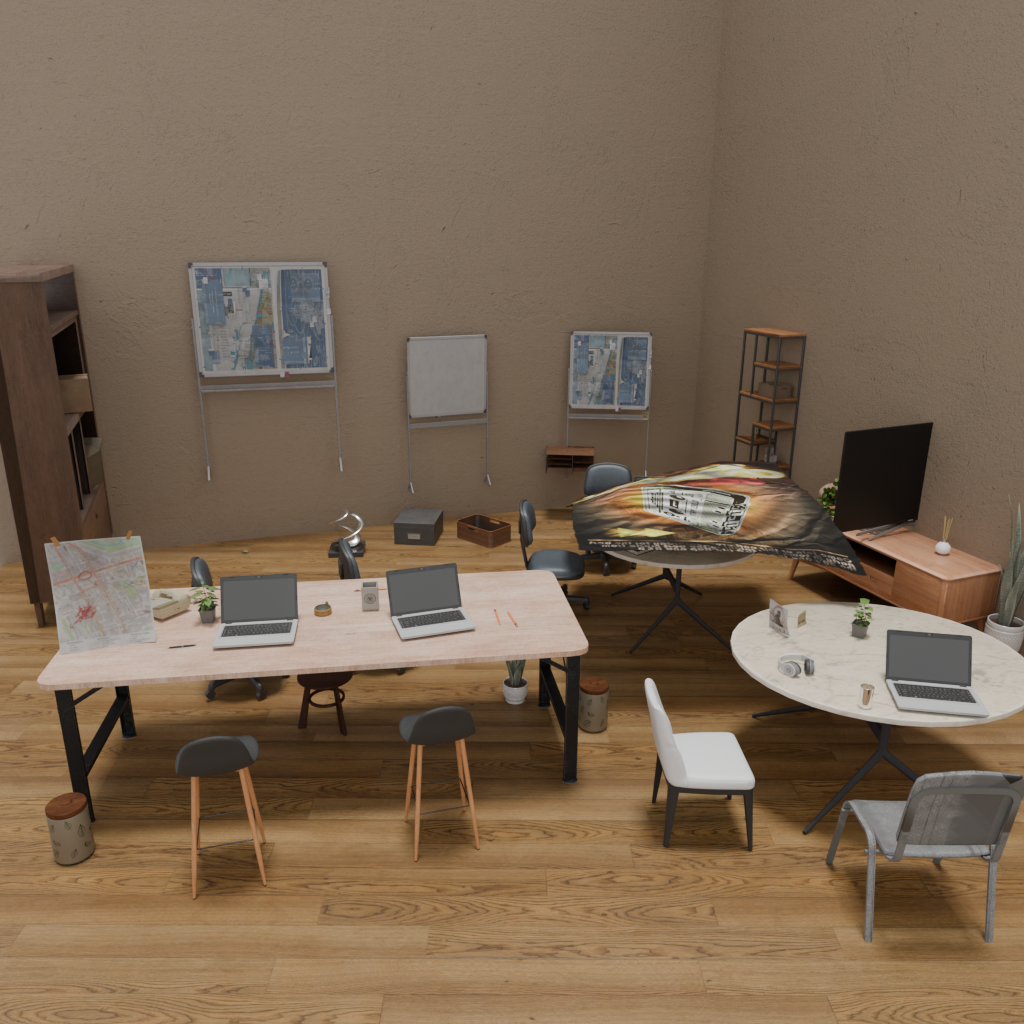
\includegraphics[width=0.235\textwidth]{../visual_results/official_v5_final.png} \\
\small (a) input image & \small (b) V1 (legacy SA) & \small (c) V3 support-aware &
\small (d) V5-fast \\
\end{tabular}
\caption{Qualitative comparison on the two hardest scenes of the benchmark,
\textsc{livingroom\_10} (top) and \textsc{official\_02} (bottom).  These are
selected as worst-case rather than best-case examples.  V1 exhibits floating
and interpenetrating objects that its stochastic refinement does not resolve;
V3 repairs support parents and stacking but still leaves collisions; V5-fast
additionally certifies contact, containment, and collision non-worsening
component-wise, so remaining defects are surfaced as unresolved rather than
silently accepted.  All three results share the same input image and, for V4
onward, the same frozen upstream S0--S3 state.}
\label{fig:qualitative}
\end{figure*}

\subsection{Failure handling and qualitative repair}

The final support/visibility layer is intentionally conservative.  It costs
166.33~s/scene on average in the current Paper30 run, trading some of Fix61's
speed advantage for true-mesh and rendered-visibility checks.  It may
accept a small true-mesh support repair only when local witnesses and aggregate
families pass; otherwise it restores the Fix61 incumbent and reports the scene
as physically or visually unresolved.  This prevents a visually appealing
single-scene edit from silently degrading the benchmark.  It also explains why
the quantitative anchor and the qualitative visual variant are recorded
together rather than conflated.

\section{Discussion}

\paragraph{Optimization and measurement must be co-designed.}
The clearest lesson from Section~\ref{sec:budget} is not that our solver is
weak but that our score is anchored.  When three of four scored families reward
agreement with the initialization, the benchmark measures \emph{fidelity plus a
quarter of improvement}, and a stronger optimizer cannot express its advantage.
This is a general hazard for single-image layout work: metrics built by
comparing against the pipeline's own initialization, or by abstaining on
relations the initialization violates, silently convert an improvement task
into a preservation task.  We report the negative result in full because the
alternative---quietly reporting only the two-step number---would leave readers
to rediscover the same wall.

\paragraph{The solver objective and the evaluator disagree in aggregation.}
Our residual uses a mean over semantic relations while the evaluator takes a
per-object maximum.  A solver can therefore reduce mean violation while
worsening an object's worst relation.  This is a concrete, addressable
mismatch, and we name it as unfinished rather than claim the aggregation is
principled.

\paragraph{Robustness is a first-class result, not a footnote.}
The first-order variant achieved a better single-scene score yet could not
complete the benchmark, because hard projection has no feasible point when the
initialization is badly wrong.  Guarded second-order iteration with bounded
relation release degrades gracefully instead.  For content pipelines, where a
single aborted scene costs an artist a full round trip, completion rate
dominates a fractional score improvement.

\paragraph{Certificates change what a failure means.}
Because \proofsys{} commits component-wise and rolls back only the owners and
separators of failed witnesses, an unrepairable defect becomes an
\emph{annotated} defect rather than a silent one.  In production this converts
debugging from visual inspection of the whole scene to reading a list of
unresolved witnesses.  We consider this, rather than the speedup, the property
most likely to transfer to other systems.

\section{Limitations and Future Work}

First, the V3 physical score has an unresolved evaluator-provenance conflict
and is excluded from the headline table.  Second, the V3 runtime is reconstructed
rather than an uninterrupted benchmark; it supports an order-of-magnitude
comparison but not a small percentage claim.  Third, exact-mesh witnesses can
abstain on open or thin meshes, and conservative rollback may retain an obvious
visual defect when no safe repair is certifiable.  Fourth, the current cached
comparison cannot isolate DeepSearch from cold-start and asset-library
confounders.  A paired S2-only experiment should freeze S1 masks, graph,
camera, seed, S3, and S4 while switching only the retriever.

Fifth, the budget conclusion of Section~\ref{sec:budget} is grid-bounded: it
covers step count, per-step translation and rotation caps, semantic weight, and
warm-start weight, but not every possible regularizer, and it is stated with
respect to an equal-weight macro that is itself initialization-anchored.
Sixth, the mean-versus-maximum aggregation mismatch between solver and
evaluator is identified but unrepaired.  Seventh, the \texttt{critical} score,
defined as the minimum over families, is identically zero on our benchmark
because some scene always zeroes some family; it currently has no
discriminative power and should be replaced by a per-family floor or a
quantile.  Eighth, the settling and centre-of-mass projection route remains
disabled by design: it repairs vertical contact only if the object dimensions
are already correct, and in three of five inspected scenes the settling target
had both wrong identity and wrong size, so settling would anchor the error
instead of removing it.  It may be reopened once retrieval scale is corrected.

Our next operating point, V5-best, will run three cold starts and choose the
best fully certified result.  Selection must use only test-time observable
evidence and must report its roughly threefold upstream compute.  Because S1
accounts for 69.6\% of cold S0--S3 compute, it---not the refinement
stage---is the correct target for further end-to-end speedup; reducing
\method{} or Fix114 time alone cannot deliver the largest gain.  If schedule
permits, Flux fine-tuning will be evaluated afterward as a separate image-prior
ablation, rather than silently altering the V5-fast benchmark.

\section{Conclusion}

We presented a two-stage evolution of a vision-guided 3D layout system.  V3
adds conservative support analysis and obtains the best recovered-object rate
in our 30-scene evaluation.  V5 replaces stochastic SA refinement with a typed,
relation-conditioned $\mathrm{SO}(3)$ LM solver and executable no-harm
certificates.  The resulting V5-fast backend raises physical quality by
7.52 points over its frozen DeepSearch source while leaving that source's pose
metrics essentially unchanged, at $3.513\times$ the speed of legacy S4 for its
core solver.  A systematic budget study then shows that this operating point is
already optimal, and explains why: early stopping functions as a trust region
on the initialization, and the benchmark's equal family weighting makes further
optimization negative-expectation.  The broader lesson is that optimization and
verification should share a typed relation contract---the solver may propose,
but only witnessed, non-inferior components may commit---and that the
evaluation must be designed to reward the improvement one intends to measure.

\paragraph{Acknowledgments.}
This work builds on Imaginarium~\cite{zhu2025imaginarium}.  We thank our
advisor and the Tencent team for the DeepSearch asset-retrieval contribution
integrated into the pipeline, which indexes on the order of $10^5$ assets with
sub-second query latency.  We will expand individual contributions and
affiliations in the camera-ready version.

\begin{thebibliography}{9}

\bibitem{zhu2025imaginarium}
X. Zhu, X. Huang, Q. Xie, Z. Deng, J. Yu, Y. Guan, Z. Liu, L. Zhu,
Q. Zhao, L. Liu, and L. Zeng.
\newblock Imaginarium: Vision-guided high-quality 3D scene layout generation.
\newblock \emph{arXiv preprint arXiv:2510.15564}, 2025.

\bibitem{levenberg1944}
K. Levenberg.
\newblock A method for the solution of certain non-linear problems in least
squares.
\newblock \emph{Quarterly of Applied Mathematics}, 2(2):164--168, 1944.

\bibitem{marquardt1963}
D. W. Marquardt.
\newblock An algorithm for least-squares estimation of nonlinear parameters.
\newblock \emph{Journal of the Society for Industrial and Applied
Mathematics}, 11(2):431--441, 1963.

\end{thebibliography}

\end{document}
